\documentclass[11pt]{article}
\usepackage{geometry}                % See geometry.pdf to learn the layout options. There are lots.
\geometry{a4paper}                   % ... or a4paper or a5paper or ... 
%\geometry{landscape}                % Activate for for rotated page geometry
%\usepackage[parfill]{parskip}    % Activate to begin paragraphs with an empty line rather than an indent
\usepackage{graphicx}
\usepackage{amsmath}
\usepackage{amssymb}
\usepackage{epstopdf}
\usepackage{verbatim}
\usepackage{url}

\DeclareGraphicsRule{.tif}{png}{.png}{`convert #1 `dirname #1`/`basename #1 .tif`.png}


\title{Assignment 3: Hidden Markov Models}
\author{\textbf{Your name here}}
\date{}                                           

\begin{document}
\maketitle
\section{Task 1}

Example equations: 
\begin{equation}
\int_0^\infty e^{-x^2} dx=\frac{\sqrt{\pi}}{2}    
\end{equation}

This is how you can align equations that span multiple rows:

\begin{align}
\mathcal{L}^{-1}\left\{f(d)\right\} &= \mathcal{L}^{-1}\left\{f_1(\delta).f_2(\delta)\right\} \\
& = \exp(mt) \star \left\{\frac{l}{2\sqrt{\pi t^3}} \exp(-l^2/{4t})\right\} \\
& = F_1 * F_2
\end{align}

\begin{align}
A &= b \\
& = c \\
& = 1234
\end{align}

In case you want to have a single number for the equation:

\begin{align}
\begin{split}
  a &= b \\
  &=c \\
  &=d \\
  &=e
\end{split}
\end{align}

\section{Task 2}

\begin{figure}[!htb]
    \centering
    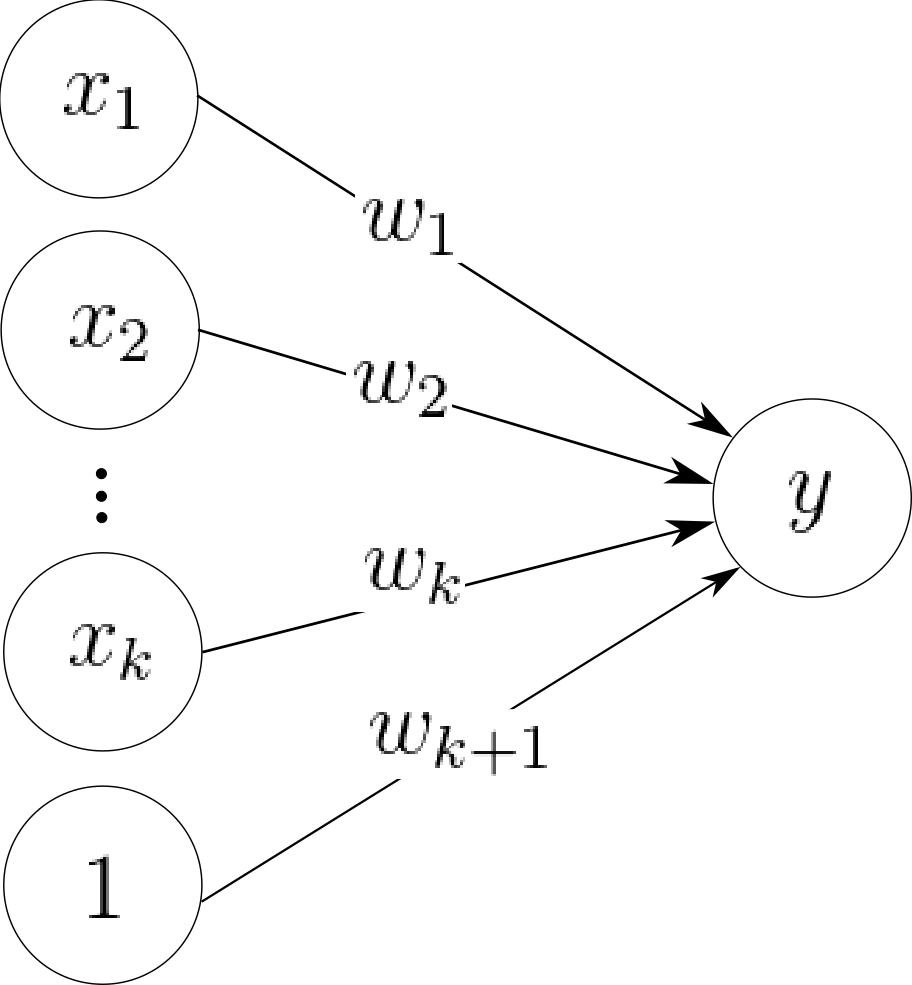
\includegraphics[width=3cm]{Perceptron.png}
    \caption{Linear perceptron.}
    \label{fig:my_label}
\end{figure}

This how you cite Figure \ref{fig:my_label}.

\section{Task 3}
This is how you cite a book, for example \cite{Bishop:2006:PRM:1162264}.\\
This is how you cite a website \cite{quoraSVM} you might have used for your assignment.

\bibliography{biblio}
\bibliographystyle{unsrt}
\end{document}  

















